\section{Power Amplifier}

\subsection{Receiver Switch}
Before building the power amplifier itself,a receiver switch was installed in order
to protect the receiver circuitry for when the transmitter will be active. 
The schematic of the protective switch is shown in
Figure~\ref{fig:RxSwitch}.

\begin{figure}[h!]
  \centering
  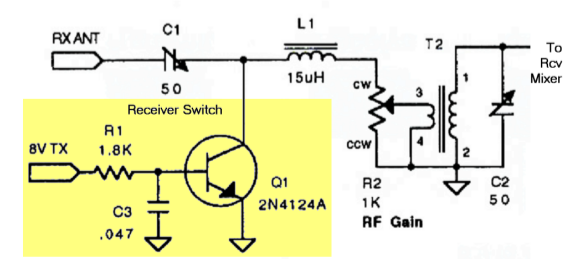
\includegraphics[scale=0.8]{./img/RxSwitch.png}
  \label{fig:RxSwitch}
  \caption{Receiver Switch}
\end{figure}

After the installation of the switching circuitry, the power amplifier was then
build according to the schematic shown in Figure~\ref{fig:powamp}.

\begin{figure}[h!]
  \centering
  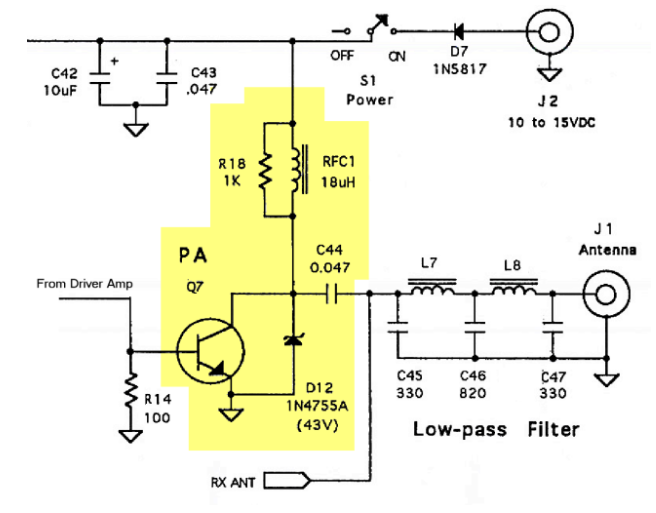
\includegraphics[scale=0.7]{./img/powamp.png}
  \label{fig:powamp}
  \caption{Power Amplifier}
\end{figure}

\subsection{Measurements and Analysis}
In order to prevent cooking the oscilloscope prematurely, a 40dB attenuator was connected
between the antenna terminal and the coaxial cable. After this, the function
generator was connected across $R_{14}$ and set initially to 1$V_{pp}$ at
7.04$MHz$.

The following conditions were noted:
\begin{align*}
  \text{Input Voltage} &\equiv        V_0[V_{pp}]\\
  \text{Output Voltage} &\equiv       V[V_{pp}]\\
  \text{Supplied Current} &\equiv     i_0[mA]\\
  \text{Supplied Power} &\equiv       P_0[mW]\\
  \text{Output Power} &\equiv         P[mW]\\
  \text{Gain} &\equiv                 G\\
  \text{Efficiency} &\equiv           \eta\\
\end{align*}
The measurable values are $V_0$, $V$, and $i_0$. The remaining values were
calculated using the following equations:
\begin{align*}
  \text{Let } & R_L=50\Omega;\, V_{DC}=12V\\
  P_0   &=  V_{DC}\cdot i_0\\
  P     &=  \frac{V^2}{16\cdot R_L}\\
  \eta  &=  \frac{P}{P_0}\\
  G     &=  20log \bigg( \frac{V}{V_0} \bigg)
\end{align*}

Ranging from 5V to 30V in increments of 2.5$V$, the relevant values were
recorded into the following table.

\begin{tabular}{|c|c|c|c|c|c|c|}
  \hline
  $V_0$   &   $V$   &   $i_0$   &   $P_0$   &   $P$   &   $G$   &   $\eta$\\
  1.712   &   5.12  &   41      &   492     &   32.7  &   9.52  &   6.7\% \\
  1.712   &   5.12  &   41      &   492     &   32.7  &   9.52  &   6.7\% \\
  1.712   &   5.12  &   41      &   492     &   32.7  &   9.52  &   6.7\% \\
  1.712   &   5.12  &   41      &   492     &   32.7  &   9.52  &   6.7\% \\
  1.712   &   5.12  &   41      &   492     &   32.7  &   9.52  &   6.7\% \\
  1.712   &   5.12  &   41      &   492     &   32.7  &   9.52  &   6.7\% \\
  1.712   &   5.12  &   41      &   492     &   32.7  &   9.52  &   6.7\% \\
  1.712   &   5.12  &   41      &   492     &   32.7  &   9.52  &   6.7\% \\
  1.712   &   5.12  &   41      &   492     &   32.7  &   9.52  &   6.7\% \\
  1.712   &   5.12  &   41      &   492     &   32.7  &   9.52  &   6.7\% \\
  1.712   &   5.12  &   41      &   492     &   32.7  &   9.52  &   6.7\% \\
  \hline

\end{tabular}

\subsection{Plotting $\eta$ v.s. $P$}

In Figure~\ref{fig:efficiencyvpower}, the efficiency $\eta$ is plotted against the
output power $P$. In Figure~\ref{fig:gainvRFvolt}, the gain of the power
amplifier was plotted against the input RF Voltage.

\begin{figure}[h!]
  \centering
  %\includegraphics[scale=0.5]
    \label{fig:efficiencyvpower}
    \caption{Plot of Efficiency $\eta$ v.s. Output Power $P$}
\end{figure}

\begin{figure}[h!]
  \centering
  %\includegraphics[scale=0.5]
    \label{fig:gainvRFvolt}
    \caption{Plot of Gain v.s. input RF Voltage}
\end{figure}
